\documentclass[10pt]{article}
\usepackage[utf8]{inputenc}

%Márgenes y tipo de hoja
\usepackage{geometry}
\geometry{letterpaper,portrait,
rmargin=20mm, 
lmargin=20mm,
bmargin=20mm,
tmargin=0mm,
headheight=0mm}
% \renewcommand{\headrulewidth}{1pt}
\usepackage{graphicx}
\usepackage{wrapfig}
\usepackage{float}

% Logos
\usepackage{fontawesome}

%Header
\usepackage{xcolor}
\usepackage{fancyhdr}
\pagestyle{fancy}
\fancyhf{}

% Tipo de letra y color
\usepackage{PTSansNarrow} 
\renewcommand*\familydefault{\sfdefault}
\usepackage[T1]{fontenc}
\usepackage{xcolor}
\usepackage{anyfontsize}

% Indentacion de parrafos completos
\usepackage{changepage}

% Paquete para columnas multiples
\usepackage{multicol}
\setlength{\columnsep}{40pt}
 \usepackage{vwcol} 

% Indentacion y otras longitudes
\setlength{\parindent}{0pt}
\setlength{\parskip}{10pt}
\renewcommand{\baselinestretch}{1}

% Figura
\usepackage{tikz}

% Hipervinculos
\usepackage{hyperref}

\begin{document}

\begin{tikzpicture}[remember picture,overlay]
   \node[anchor=north,inner sep=0pt] at (current page.north)
  \draw[blue, very thick] (-5,-3.1) rectangle (50,5);
  \filldraw[fill=blue!50!black, draw=blue!50!black](-5,-3.1) rectangle (50,5);
\end{tikzpicture}
\begin{tikzpicture}[remember picture,overlay]
    \node[anchor=north east,inner sep=0pt] at (current page.north east)
    {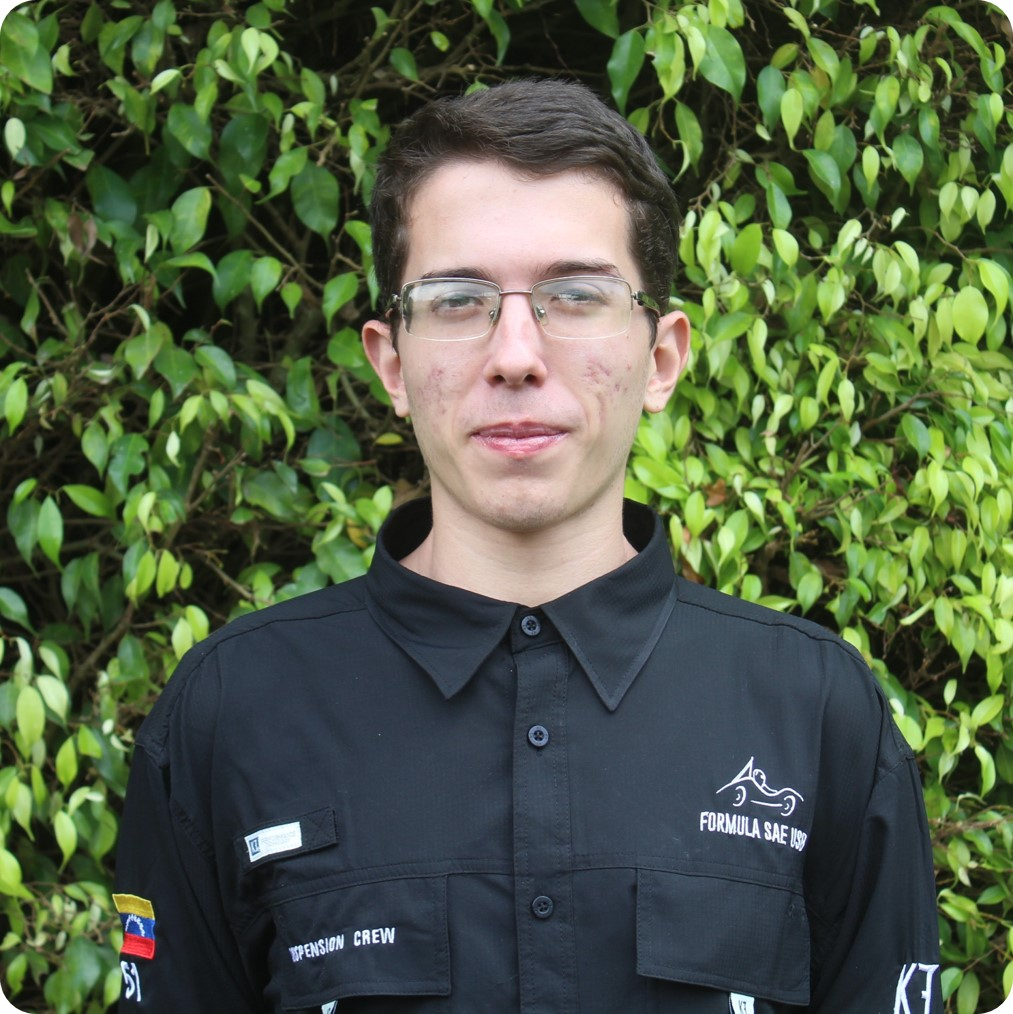
\includegraphics[scale=0.2]{foto/foto_perfil.JPG}};
\end{tikzpicture}

\begin{center}
    \color{white}
    {\fontsize{40}{60}\selectfont Jesús \textbf{Pereira}}\vspace{4pt}\\
    \faMapMarker\hspace{3pt}Caracas\hspace{5pt}/\hspace{5pt}Venezuela\hspace{25pt}| \hspace{25pt}\faMobile\hspace{2pt} +58 424 1234715\hspace{25pt}|
    \hspace{25pt}\faChain\hspace{2pt}\href{https://jesusepp.github.io/}{jesusepp.github.io}\\\vspace{2pt}
    \faEnvelope\hspace{2pt}jesusepereira@gmail.com\hspace{25pt}|
    \hspace{25pt}\faLinkedinSquare\hspace{3pt}\href{https://www.linkedin.com/in/jeppires/}{/in/jeppires/}\hspace{25pt}|
    \hspace{25pt} \faGithubSquare\hspace{3pt}\href{https://github.com/jesusepp}{/jesusepp}
\end{center}

\vspace{20pt}

\begin{multicols}{2}
    \begin{LARGE}
        \color{blue!50!black}Skills\par
    \end{LARGE}
    \begin{vwcol}[widths={0.4,0.6},
 sep=0cm,rule=0pt,indent=0em,lines=9]
        \textbf{Programming Languages}\par\hfill\\\hfill\\
        \textbf{Other Languages}\par\hfill\\
        \textbf{Programs and Platforms}\par\hfill\\\hfill\\\hfill\\
        MATLAB, Python, JavaScript PHP, SQL, C++.\par\hfill\\
        Tex, HTML, CSS.\par\hfill\\
        SolidWorks, ANSYS Mechanical, ANSYS Fluent, MATLAB, OverLeaf, Excel, PowerPoint, Word, Google Docs.\par
    \end{vwcol}
    \columnbreak
    \begin{LARGE}
        \color{blue!50!black} Personal Information\par
    \end{LARGE}
    Currently I'm a 10th trimester, Mechanical Engineering student at Universidad Simon Bolivar, member of the university Formula SAE team, passionate on learning, motor sports and programming, and capable of resolving issues that require teamwork and cooperation.\par
    \begin{LARGE}
        \color{blue!50!black} Languages\par
    \end{LARGE}
    \begin{vwcol}[widths={0.235,0.765},
 sep=.8cm,rule=0pt,indent=0em,lines=4]
        \textbf{Spanish}\\
        \textbf{English}\\
        \textbf{German}\\
        \textbf{Portuguese}\\
        Native\\
        Advance\\
        Basic\\
        Basic\\
    \end{vwcol}
\end{multicols}

\begin{LARGE}
        \color{blue!50!black} Courses\par
\end{LARGE}
    
\begin{multicols}{2}
    \begin{vwcol}[widths={0.235,0.765},
 sep=.8cm,rule=0pt,indent=0em,lines=9]
        \hspace{5pt}Oct/2019\\
        \hfill\\
        \hfill\\
        \hspace{5pt}Apr/2020\\
        \hfill\\
        \hfill\\
        \hspace{5pt}May/2020\\
        \hfill\\
        \hfill\\
        CSWA, SolidWorks Associated. Credential: \href{https://cv.virtualtester.com/qr/?b=SLDWRKS&i=C-4JDU269MA5}{\textbf{C-4JDU269MA5}}\par\hfill\\
        Certification - EF-SET with 80/100. Credential: \href{https://www.efset.org/cert/oZC3oZ}{\textbf{EF-SET}}\par\hfill\\
        Introduction to Programming with MATLAB. Credential: \href{https://www.coursera.org/account/accomplishments/verify/E63RKFRUKWEU}{\textbf{E63RKFRUKWEU}}\par\hfill\\
    \end{vwcol}
    \columnbreak
    \begin{vwcol}[widths={0.235,0.765}, sep=.8cm,rule=0pt,indent=0em,lines=9]
        \hspace{5pt}Jul/2020\\
        \hfill\\
        \hfill\\
        \hspace{5pt}Jul/2020\\
        \hfill\\
        \hfill\\
        \hspace{5pt}Aug/2020\\
        \hfill\\
        \hfill\\
        Statistics with Python Specialization. Credential: \href{https://www.coursera.org/account/accomplishments/specialization/certificate/NE5BJHUXH5VM}{\textbf{NE5BJHUXH5VM}}\par\hfill\\
        Engineering Project Management Specialization. Credential: \href{https://www.coursera.org/account/accomplishments/specialization/certificate/YMNNPDXQL97L}{\textbf{YMNNPDXQL97L}}\par\hfill\\
        SQL for Data Science. Credential: \href{https://www.coursera.org/account/accomplishments/certificate/MSH6GML4W8AM}{\textbf{MSH6GML4W8AM}}\par\vspace{5px}
    \end{vwcol}
\end{multicols}

\begin{LARGE}
    \color{blue!50!black} Education\par
\end{LARGE}
\begin{multicols}{2}
     \begin{vwcol}[widths={0.4,0.6}, sep=.2cm,rule=0pt,indent=0em,lines=4]
    \hspace{5pt}Apr/2016 - Present\\
    \hfill\\
    \hfill\\
    \hfill\par
    \textbf{Mechanical Engineering}\\
    Universidad Simón Bolívar\\
    160 credits (73\% of the total)\\
    Academic Index: 4.92/5.00
    \end{vwcol}
\end{multicols}


\begin{LARGE}
    \color{blue!50!black} Previous Jobs\par
\end{LARGE}

\begin{vwcol}[widths={0.235,0.765},
 sep=.8cm,rule=0pt,indent=0em,lines=7]
    \hspace{5pt}Jul/2020 - Present\par
    \hfill\\
    \hfill\\
    \hfill\\
    \hfill\\
    \hfill\\
    \hfill\\
    \textbf{Technical Director / Chassis and Brakes Director}
    \hfill
    \href{http://fsaeusb.com.ve/}{\color{blue!50!black}\textbf{FSAE USB}}\\
    \vspace{5pt}
    As Technical Director, I'm in charged of directing and controlling the actions of the technical divisions of the team. This position requires leadership, planning and good communication with every one of the division leaders. Motor sports, vehicle dynamics, computer aided design (CAD), and computer aid engineering (CAE) are some of the technical areas that this positions requires. Additionally, this particular year, I was also in charged of the  brakes and chassis divisions.\par
\end{vwcol}
\clearpage
\hfill\\
\hfill\\

\begin{vwcol}[widths={0.235,0.765},
 sep=.8cm, rule=0pt,indent=0em,lines=8]
    \hspace{5pt}Jul/2019 - Jul/2020\par
    \hfill\\
    \hfill\\
    \hfill\\
    \hfill\\
    \hfill\\
    \hfill\\
    \hfill\\
    \textbf{Chassis Director}
    \hfill
    \href{http://fsaeusb.com.ve/}{\color{blue!50!black}\textbf{FSAE USB}}\\
    \vspace{5pt}
    As chassis director, I got the responsibility of design, build and verify a variety of systems, some of them are the frame and it's connections to the variety of other system that work together to make a functional formula SAE prototype, and the security systems that are require (all of this, building on top of the competition rule set). This division has a key role in the communication with the other  divisions, as it's responsible to develop a design that allow good synergy around all the systems.\par
\end{vwcol}

\begin{vwcol}[widths={0.235,0.765},
 sep=.8cm, rule=0pt,indent=0em,lines=6]
    \hspace{5pt}Jul/2018 - Jun/2019\par
    \hfill\\
    \hfill\\
    \hfill\\
    \hfill\\
    \hfill\\
    \textbf{Suspension Member}
    \hfill
    \href{http://fsaeusb.com.ve/}{\color{blue!50!black}\textbf{FSAE USB}}\\
    \vspace{5pt}
    This division is responsible of the design, construction and testing of the suspension system of a formula SAE prototype. During this period, I worked along side other students to achieve a functional system, acquiring knowledge over design software like SolidWorks, machining tools like lathes and milling machine, and basic mechanical standards like fasteners.\par
\end{vwcol}

\begin{LARGE}
    \color{blue!50!black} Projects\par
\end{LARGE}


\begin{vwcol}[widths={0.235,0.765},
 sep=.8cm, rule=0pt,indent=0em,lines=6] 
\hspace{5pt}Jun/2020 - Jul/2020\par
    \hfill\\
    \hfill\\
    \hfill\\
    \hfill\\
    \hfill\\
    \textbf{Web Page}\hfill \href{https://jesusepp.github.io/}{\color{blue!50!black}\textbf{jesusepp.github.io}}\\
    \vspace{5pt}
    During the period of quarantine that happened during 2020, I started to learn about web development, mainly from curiosity. But, as a personal task to practice my newly developed skills, I started this project along side my friend José, to develop a personal website that served as a more detailed and visual-friendly source of information about my self.\par
\end{vwcol}

\begin{vwcol}[widths={0.235,0.765},
 sep=.8cm, rule=0pt,indent=0em,lines=5] 
\hspace{5pt}Apr/2020\par
    \hfill\\
    \hfill\\
    \hfill\\
    \hfill\\
    \textbf{Minesweeper with Python}\hfill \href{https://github.com/jesusepp/minesweeper}{\color{blue!50!black}\textbf{/jesusepp/minesweeper}}\\
    \vspace{5pt}
    Using the Python programming language, and with the objective of practicing my new acquire skills using it (I recently did an online course of Python), I made a version for terminal of the classic minesweeper game. I believe the results were good, link to the source code provided above.\par
\end{vwcol}

\begin{vwcol}[widths={0.235,0.765},
 sep=.8cm, rule=0pt,indent=0em,lines=6] 
\hspace{5pt}Mar/2020 - Present\par
    \hfill\\
    \hfill\\
    \hfill\\
    \hfill\\
    \hfill\\
    \textbf{Curriculum}\hfill \href{https://github.com/jesusepp/Curriculum-en-LaTeX}{\color{blue!50!black}\textbf{/jesusepp/Curriculum-en-LaTeX}}\\
    \vspace{5pt}
    For practice purposes, and basically for making my own curriculum, and decided that a good place for improving my LaTeX skills was to do write it my self. It is an on going project, and you could find a link to its source code above.\par
\end{vwcol}

\begin{vwcol}[widths={0.235,0.765},
 sep=.8cm, rule=0pt,indent=0em,lines=8] 
\hspace{5pt}Jan/2020 - Apr/2020\par
    \hfill\\
    \hfill\\
    \hfill\\
    \hfill\\
    \hfill\\
    \hfill\\
    \hfill\\
    \textbf{Virtual Formula 2020}\hfill \href{https://www.vi-grade.com/en/about/virtual_formulas/virtual-formula-2020/?#virtualformula2020}{\color{blue!50!black}\textbf{vi-grade.com - 2020 Results}}\\
    \vspace{5pt}
    This is a virtual competition related with FSAE teams, and this year our team decided to take part on it (with me in charge). This is a competition based on simulating a car with the Virtual Race Car software (lap simulator), where each team had to build the faster configuration inside the regulations of the competition. We finished 20/35, been this our first time in this competition and using this software.\par
\end{vwcol}
\end{document}
